\chapter{Проектирование}
\label{cha:ch_1}

Процесс проектирования в данной работе представлен из двух частей: исследование аспектов проблематики и составление базы приёмов программной инженерии, которые будут использоваться в процессе разработки.

\section{Выбор основного способа запрашивания ввода}
Имея перед собой цель создания ассетов способных автоматизировать действия пользователя внутри разрабатываемого приложения, необходимо было выбрать самый лёгкий способ запрашивания ввода, который будет перехватываться и записываться.

Метрикой лёгкости способов запрашивания ввода здесь будет являться длина двумерного вектора из количества необходимых для использования единиц компиляции (ЕК) и количества использованных строк кода (ИСК). Далее была сформулирована нулевая гипотеза: самый лёгкий способ запрашивания ввода имеет минимальную длину вектора данной проверочной статистики и является классом Input.

Согласно официальному мануалу посвящённому системам запрашивания ввода \cite{unity_input_systems} на платформе \textit{Unity} существует два модуля подобных систем: Input Manager и Input System. Первая система включает в себя два способа: класс взятия универсального ввода Input и интерфейсы-маркеры для взаимодействия только с указателем (мышкой, пальцем и т.д.). Вторая система, по сути своей, является альтернативой первой, она поставляется отдельно, требует установки дополнительных зависимостей и содержит единственный способ взятия ввода путём создания специальных профилей, где описывается ассоциация определённого объекта в памяти с потоком данных из определённого периферийного устройства.

Для того чтобы определить количество единиц компиляции, выражение на языке программирования CSharp (основном языке платформы \textit{Unity}) переписывается с использованием классов пространства имён \textit{System.Reflection} стандартной библиотеки CSharp. Количество экземпляров классов задействованных в переписанной версии выражения и будет являться количеством единиц компиляции.

Для подсчёта ЕК и ИСК в интерфейсе-маркере использовался пример из Unity Scripting API \cite{unity_interface}, а для Input System использовался пример из Unity Manual \cite{unity_is}.

\begin{table}[H]
	\caption{\label{tab:inputs}Таблица векторов данных и их длин}
	\begin{center}
		\begin{tabular}{|c|c|c|c|}
			\hline
			& \multicolumn{2}{c|}{Количество} & Метрика \\
			\cline{2-4}
			\raisebox{1.5ex}[0cm][0cm]{Способ запрашивания ввода}
			& ЕК & ИСК & Длина вектора \\
			\hline
			Класс Input & 3 & 1 & $\sqrt{3^2+1} = \sqrt{10}$ \\
			\hline
			Интерфейс-маркер & 6 & 4 & $\sqrt{6^2+4^2} = \sqrt{44}$ \\
			\hline
			Input System & 7 & 6 & $\sqrt{7^2+6^2} = \sqrt{85}$ \\
			\hline
		\end{tabular}
	\end{center}
\end{table}

Опираясь на данные приведённые в таблице \ref{tab:inputs} можно утвердить нулевую гипотезу. Однако, всего вышесказанного недостаточно, чтобы сделать окончательный выбор и остановиться на классе Input. Данный вывод лишь указывает на необходимое условие критерия выбора способа запрашивания ввода. Теперь же нужно предоставить достаточное условие.

Достаточным условием выбора класса Input в качестве основы для перехвата и записи является то, что этот инструмент популярен и распространён среди других Unity-проектов. Теперь формируем следующую нулевую гипотезу: математическое ожидание количества использований класса Input в кодовой базе любого проекта на \textit{Unity} больше нуля.

Другими словами, в среднем по всем значимым проектам количество использований класса Input будет больше нуля. Это будет указывать не только на популярность использования данного способа, но и на распространённость, ведь создавая новый продукт, каждый разработчик старается опираться на лучший опыт других значимых проектов и это выражается в виде существования библиотек для ПО, фреймворков и др.

Генеральной совокупностью в рамках данной работы принято считать все Unity-проекты с максимальным количеством использования CSharp (т.е доля языка CSharp в проекте доминирует), с максимальным количеством форков (проектов, в основе которых лежит выбранный проект), со стабильным обновлением и с максимальной поддержкой своих сообществ. 

Далее была произведена выборка проектов с помощью реализованной в рамках данной работы spider-программы описанной в начале второй главы. Структура выборки наглядно иллюстрируется в таблице \ref{tab:sample}. Размер выборки составляет 3970 проектов из 99509 возможных по запросу ``language:csharp unity'' на сайте GitHub.com. Ввиду технических ограничений данного сайта, существует возможность исследовать только столько проектов, сколько составляет размер описанной выборки.

\begin{table}[H]
	\caption{\label{tab:sample}Структура выборки с количеством использований класса Input}
	\begin{center}
		\begin{tabular}{|c|c|c|}
			\hline
			& \multicolumn{2}{c|}{Извлечённые данные} \\
			\cline{2-3}
			\raisebox{1.5ex}[0cm][0cm]{Название проекта}
			& Количество исп. & Номер \\
			\hline
			github-for-unity/Unity & 1 & 0 \\
			\hline
			Unity-Technologies/UnityCsReference & 0 & 1 \\
			\hline
			XINCGer/Unity3DTraining & 62 & 2 \\
			\hline
			... & ... & ... \\
			\hline
			KuraiAndras/MainThreadDispatcher.Unity & 0 & 3969 \\
			\hline
		\end{tabular}
	\end{center}
\end{table}

Итак, данные собраны. Для наглядной оценки математического ожидания количества использований, был выбран бутстраповский доверительный интервал \cite{oreilly} с уровнем доверия 90\%. Алгоритм просчёта границ интервала довольно прост:

\begin{itemize}
	\item Определяем размер выборки $n$ и некоторое большое число $R$;
	\item далее извлекаем случайную выборку размера $n$ с возвратом из данных (повторная выборка);
	\item записать целевую статистику для повторной выборки;
	\item повторить предыдущие шаги $R$ раз;
	\item для $x$-процентного доверительного интервала отсечь $\left[(1-\left[x / 100\right])/2\right]\%$ от $R$ результатов слева и справа;
	\item точками отсечения являются конечные точки $x$-процентного бутстраповского доверительного интервала.
\end{itemize}

Для данной работы, параметру $R$ было присвоено значение 99509, как если бы техническое ограничение источника данных на длину выборки отсутствовало, а параметрам $n$ и $x$ присвоены значения 3970 и 90 соответственно. Результаты подсчёта интервальной оценки иллюстрируются на рис. \ref{experiment}, где ось абсцисс -- номер повторной выборки, а ось ординат -- выборочное математическое ожидание.

\begin{figure}[H]
	\centering
	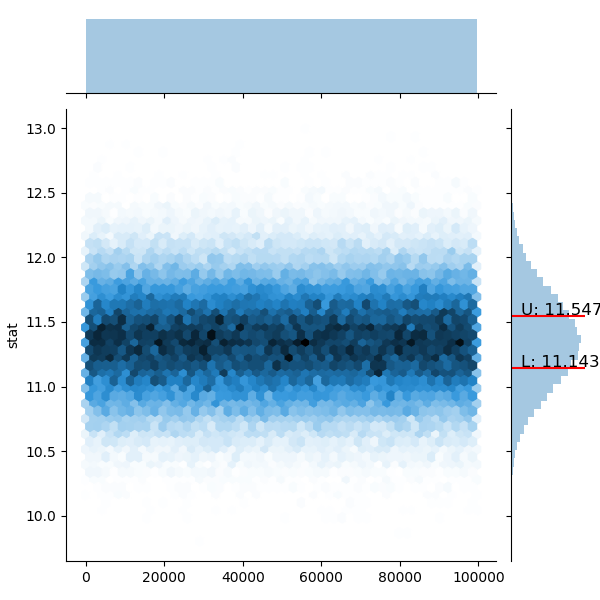
\includegraphics[width=\linewidth]{experiment.png}
	\caption{Диаграмма рассеивания бутстраповской интервальной оценки}
	\label{experiment}
\end{figure}

Основываясь на данных полученных в результате подсчёта описанного выше доверительного интервала, можно с уверенностью 90\% утвердить нулевую гипотезу, так как полученные границы находятся выше нуля и равны 11.143 и 11.547 соответственно.

\section{Класс совместимых приложений}
Разработанная в рамках данной работы группа ассетов имеет название Automated Test Framework (ATF) и может быть интегрирована c любым  \textit{Unity}-проектом, система ввода которого построена вокруг класса из стандартной библиотеки \textit{Unity} по запрашиванию ввода Input. Под это описание подходит большая часть \textit{Unity}-приложений, как было обосновано в предыдущем разделе.

\section{Определение теоретической базы}
В основе проектирования сложных ассетов всегда необходимо учитывать фундаметальные принципы построения ПО с использованием объектно-ориентированного подхода. Этими принципами в рамках описываемого процесса разработки являются пять правил SOLID \cite{solid}, принцип ухода от повторений единиц компиляции и интерпретации DRY \cite{dry}, а также принцип лезвия Оккама, который позволяет избежать избытка разрабатываемых сущностей в виде классов. Дополнительными особенностями данной кодовой базы можно назвать автоматическую систему переноса и упаковки группы ассетов, характерную для \textit{Unity}-платформы (``.unitypackage'' пакетирование), а также возможность автоматической интеграции в исходный код любого Unity-проекта, где будет использован предмет данной разработки.

\begin{figure}[H]
	\centering
	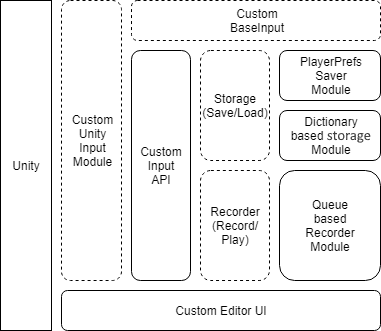
\includegraphics[width=0.6\linewidth]{platform.png}
	\caption{Диаграмма платформы решения}
	\label{platform}
\end{figure}

На этапе проектирования была составлена диаграмма платформы (см. рис. \ref{platform}), каждый блок которой -- это изолированная группа методов API, решающая свои задачи: 
\begin{itemize}
	\item \textit{Unity} -- непосредственно сам игровой движок;
	\item \textit{Custom Unity Input Module} -- абстракция, объединяющая управление вводом;
	\item \textit{Custom Input API} -- собственно API, который вызывает нативные методы по запросу ввода;
	\item \textit{Custom BaseInput} --  сущность, которая является реализацией объекта обработки потока данных через мост (Bridge), объединяя статичные методы по перехвату/симуляции ввода и обернутые события (Events);
	\item \textit{Storage} --  абстракция, отвечающая за функционал хранения и манипуляции записанных действий;
	\item \textit{Recorder} -- абстракция, отвечающая за запись действий;
	\item \textit{Custom Editor UI} -- система пользовательских окон для управления всеми процессами;
	\item \textit{PlayerPrefs Save/Load Module} -- система реализации абстракции модуля по сохранению/загрузке записанных действий на базе стандартного класса PlayerPrefs;
	\item \textit{Dictionary based Module} -- реализация абстракции хранилища записанных действий, основанная на структуре данных ``Словарь'';
	\item \textit{Queue based Recorder Module} -- реализация абстракции, отвечающей за запись действий, основанная на структуре данных ``Очередь''.
\end{itemize}

Для выполнения поставленных задач было разработано решение, являющееся, по своей сути, модифицированным адаптером, который перехватывает и симулирует ввод. Для его эффективной реализации стало органичным использовать несколько архитектурных паттернов:
\begin{itemize}
	\item
	\textit{Interceptor} -- шаблон для перехвата и подмены входных данных с периферийных устройств \cite{interceptor};
	\item
	\textit{Broker} -- шаблон для интеграции и взаимодействия с встроенной системой управления входными данными \textit{Unity} \cite{broker};
	\item
	\textit{PAC (Presentation–abstraction–control)} -- шаблон для организации взаимодействия зависимых систем \cite{pac}.
\end{itemize}

Для подмены стандартного класса Input был создан перехватчик класс ATFInput (см. рис. \ref{atfInput}). Данный класс наследуется от класса MonoSingleton<ATFInput>, который является специальной реализацией паттерна Singleton для объектов на сцене. Также перехватчик имплементирует интерфейс IBaseInput, который объединяет в себе интерфейсы Input класса и стандартного класса BaseInput. Данное объединение необходимо для того, чтобы обеспечить полноту копирования интерфейса класса Input, одновременно сохраняя совместимость с системой распределения события Unity. 

\begin{figure}[H]
	\centering
	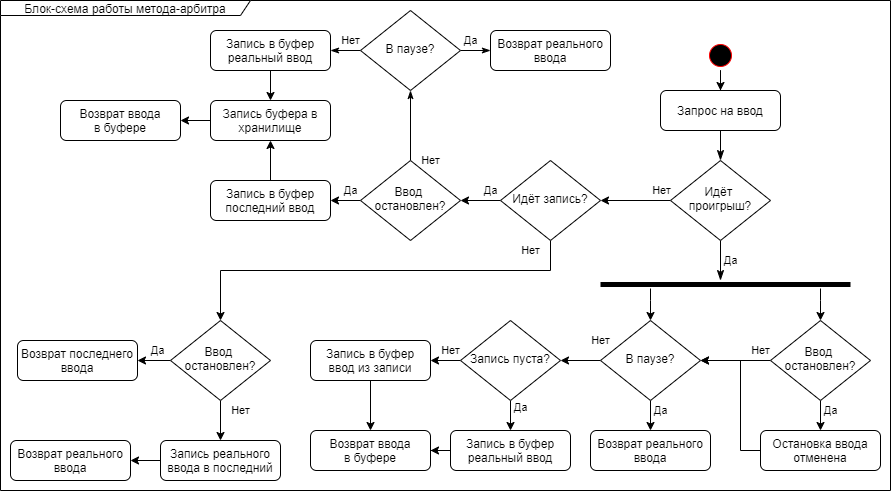
\includegraphics[width=\linewidth]{rofior_diagram.png}
	\caption{Блок-схема деятельности метода-арбитра ATFInput}
	\label{atfInput}
\end{figure}

Стоит заметить, что под ``Запросом на ввод'' имеется ввиду вызов любого метода класса ATFInput, который повторяет сигнатуру метода класса Input. Некоторые из методов класса ATFInput также доступны по объектному доступу. Именно это оставляет совместимость ATFInput со стандартным компонентом Event System, потому как данный компонент обращается к методам перехватчика по объектному доступу.

Для интерпретации (проигрывания) первоначально использовался паттерн Interpreter с терминалами ожидания внутри Coroutine. Однако после попытки тестовой реализации данного шаблона был произведен отказ в пользу метода записи, основанного на структуре данных ``Очередь'', так как для правильной работы терминалов ожидания необходимо было просчитывать заранее действия пользователя, что значительно усложнило бы задачу.